\chapter{Introduction}
\label{chap:Introduction}
This report presents the results of the project “Visualizing the Netherlands” as part of the course “Additional component computer graphics”. The goal of the project was to design and implement a system which is able to visualize the Netherland based on the BAG-extract \cite{BAG14} and other open data sources. The BAG-extract is a data set that contains information on all the buildings and addresses in the Netherlands. A screenshot of a rendered image is in \ref{fig:utrechtCenter}

\begin{figure}[htb!]
\centering
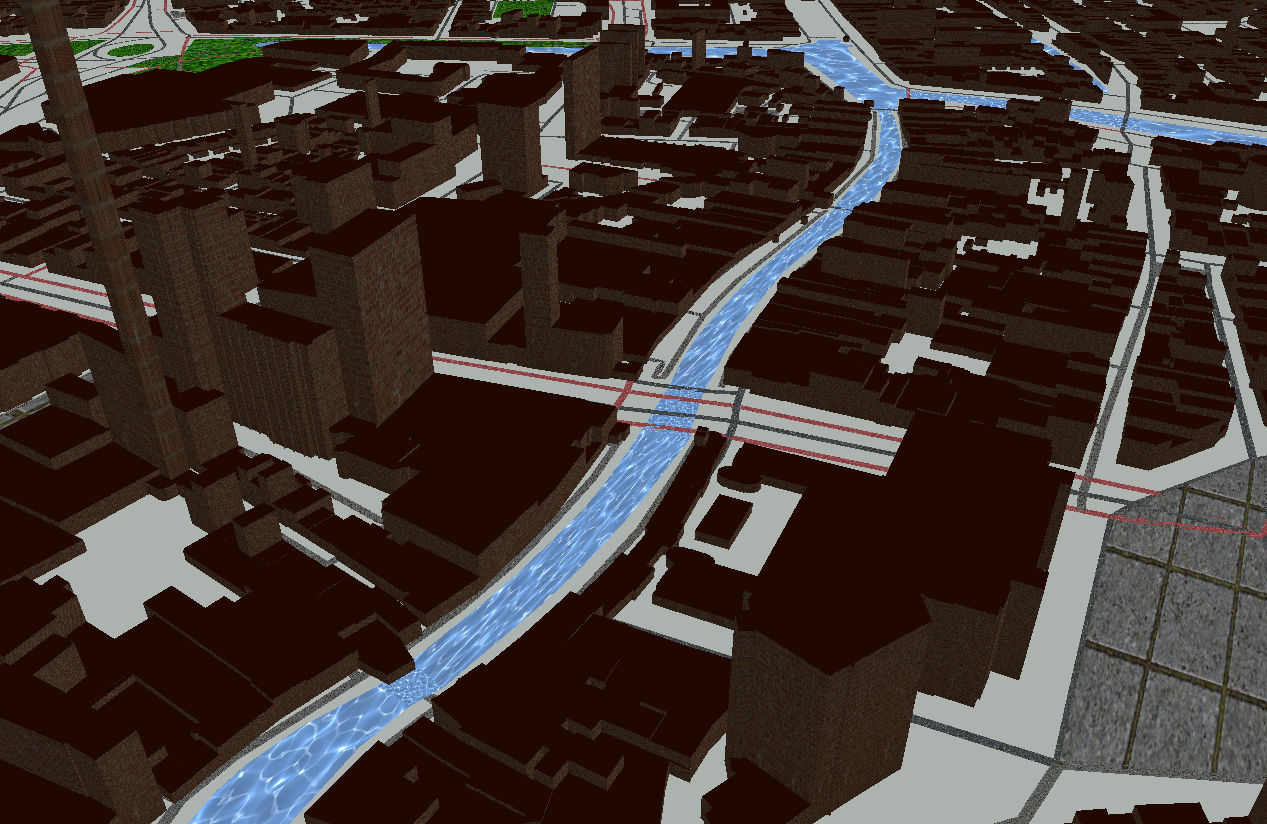
\includegraphics[width=0.6\textwidth]{CenterUtrecht}
\caption{Center of Utrecht}
\label{fig:utrechtCenter}
\end{figure}

Firstly, the report presents the main challenges of the project. Secondly, in section \ref{chap:OpenDataSets} the open data sets used will be presented. Then the requirements and the desired functionality of the system are described in section \ref{chap:Requirements}. Related works, which helped us solving the project’s challenges, are presented in section \ref{chap:DiscussionOfLiterature}. In the literature study, methods to construct and visualize large worlds out of large data sets have been researched. Then in section \ref{chap:AnalysisAndSolution}, a short analysis of the used data sets is made and the system design and algorithms used are presented. The system uses specific data structures and methods to access the out-of-memory data set. Algorithms to construct and to use these data structures are also presented. Furthermore, in section \ref{chap:ResultsAndEvaluation} the results of the implementation of the designed system and algorithms are discussed. Here the implemented system will be tested in various scenarios to see how the system performs. Finally a conclusion on the results is made and possible improvements or extensions on the systems are proposed in section \ref{chap:ConclusionAndFutureWork}.

